\documentclass[a4paper,12pt]{report}
\usepackage[utf8]{inputenc} % this is needed for fr umlauts
\usepackage[french]{babel} % this is needed for fr umlauts
\usepackage[T1]{fontenc}    % this is needed for correct output of umlauts in pdf
\usepackage{textcomp}
\usepackage[margin=2.5cm]{geometry} %layout
\usepackage[usenames,dvipsnames,svgnames,table]{xcolor}
\usepackage[pdftex,urlcolor=blue,pdfstartview=FitH]{hyperref}
% \usepackage{hyperref}  
\usepackage{listings} 
\usepackage{graphicx}
\usepackage{subfig}
\usepackage{array}
\usepackage[section]{placeins}
\usepackage[usenames,dvipsnames,svgnames,table]{xcolor}
% \usepackage[pdftex,urlcolor=blue,pdfstartview=FitH]{hyperref}

\usepackage[ %quotation package
    left = \flqq,% 
    right = \frqq,% 
    leftsub = \flqq,% 
    rightsub = \frqq%
]{dirtytalk}

\lstset{ %
  language=Python,                  % the language of the code
  basicstyle=\footnotesize,       % the size of the fonts that are used for the code
  numbers=left,                   % where to put the line-numbers
  numberstyle=\tiny\color{gray},  % the style that is used for the line-numbers
  stepnumber=1,                   % the step between two line-numbers. If it's 1, each line 
                                  % will be numbered
  numbersep=5pt,                  % how far the line-numbers are from the code
  backgroundcolor=\color{white},  % choose the background color. You must add \usepackage{color}
  showspaces=false,               % show spaces adding particular underscores
  showstringspaces=false,         % underline spaces within strings
  showtabs=false,                 % show tabs within strings adding particular underscores
  frame=single,                   % adds a frame around the code
  rulecolor=\color{black},        % if not set, the frame-color may be changed on line-breaks within not-black text (e.g. commens (green here))
  tabsize=4,                      % sets default tabsize to 2 spaces
  % captionpos=b,                   % sets the caption-position to bottom
  breaklines=true,                % sets automatic line breaking
  breakatwhitespace=false,        % sets if automatic breaks should only happen at whitespace
  title=\lstname,                 % show the filename of files included with \lstinputlisting;
                                  % also try caption instead of title
  keywordstyle=\color{blue},          % keyword style
  commentstyle=\color{olive},       % comment style
  stringstyle=\color{violet},         % string literal style
  escapeinside={\%*}{*)},            % if you want to add a comment within your code
  morekeywords={*,...}               % if you want to add more keywords to the set
}
%%%%%%%%%%%%%%%%%%%%%%%%%%%%%%%%%%%%%%%%%%%%%%%%%%%%%%%%%%%%%%%%%%%%%%
% Variablen                                                          %
%%%%%%%%%%%%%%%%%%%%%%%%%%%%%%%%%%%%%%%%%%%%%%%%%%%%%%%%%%%%%%%%%%%%%%
\newcommand{\authorName}{Pierre Labadille}
\newcommand{\tags}{\authorName, tensorflow, keras, convnet, neural-network, food-classification, M2-DNR2i}
\title{Rapport de projet tuteuré : Reconnaissance automatique d'image de plat}
\title{%
  \begin{figure}[!h]%
    \centering
    
\includegraphics[width=5cm]{img/unicaen.jpg}%
  \end{figure}%
  Rapport de projet tuteuré : Reconnaissance automatique d'image de plat \\
  \large Sujet proposé par Marc Houssaye, directeur de MH-COMMUNICATION \\
  \large Encadré par François Rioult, enseignant-chercheur UCBN (GREYC) \\
    Université de Caen Normandie - M2-DNR2i \\
    Code visualisable sur \href{https://github.com/plabadille/cookedDishRecognizer}{github}
}
\author{\authorName}
\date{\today}

%%%%%%%%%%%%%%%%%%%%%%%%%%%%%%%%%%%%%%%%%%%%%%%%%%%%%%%%%%%%%%%%%%%%%%
% PDF Meta information                                               %
%%%%%%%%%%%%%%%%%%%%%%%%%%%%%%%%%%%%%%%%%%%%%%%%%%%%%%%%%%%%%%%%%%%%%%
\hypersetup{
  pdfauthor   = {\authorName},
  pdfkeywords = {\tags},
  pdftitle    = {rapport_ptut2017}
} 

%%%%%%%%%%%%%%%%%%%%%%%%%%%%%%%%%%%%%%%%%%%%%%%%%%%%%%%%%%%%%%%%%%%%%%
% THE DOCUMENT BEGINS                                                %
%%%%%%%%%%%%%%%%%%%%%%%%%%%%%%%%%%%%%%%%%%%%%%%%%%%%%%%%%%%%%%%%%%%%%%
\begin{document}
  \maketitle
  \tableofcontents

  \chapter{Introduction}
  Le domaine du web est un secteur d'innovation et d'évolution très rapide. La quantité de données, d'applications et d'informations y croit de façon exponentielle depuis plusieurs années.
  \medbreak
  \say{ \emph{Chaque seconde, 29.000 Gigaoctets (Go) d'informations sont publiés dans le monde, soit 2,5 exaoctets par jour soit 912,5 exaoctets par an. Un volume de "big data" qui croît à une vitesse vertigineuse et donne naissance à de nouveaux types de statistiques.} \textbf{\href{<http://www.planetoscope.com/Internet-/1523-informations-publiees-dans-le-monde-sur-le-net-en-gigaoctets-.html>}{ - planetoscope.com}} }
  \medbreak
  Comme l'indique ces statistiques, cette masse de données ainsi que les évolutions des systèmes de crawling\footnote{Crawl: récupération automatique de contenu} induisent de nouvelles problématiques: il n'est aujourd'hui plus possible, sans des ressources considérables, de vérifier et assembler des données à la main sur des systèmes basés sur du crawl automatique.

    \section{Présentation du projet}
    RestoFolio est une application web innovante proposant de trouver un restaurant par le biais d’un plat précis ou plutôt grâce à une photo de celui-ci.
    \medbreak
    Actuellement, Restofolio récupère des données (images et informations) de milliers de restaurants à l'échelle de la France entière toutes les nuits. Précédemment, l'application n'opérait qu'à une échelle locale (quelques villes de la région) et la validation de ces images était manuelle. Cette validation qui n'était déjà pas optimale à petite échelle est donc aujourd'hui impossible.
    \medbreak
    La solution à court terme qui a été choisie est l'utilisation de l'API Vision de Google\footnote{Plus d'information sur cette API plus tard dans le rapport} qui offre un système de classification automatique d'image performant. Cependant elle a également des limites: l'utilisation de cette dernière n'est pas gratuite, elle n'est pas contrôlée par l'entreprise (mais par un service extérieur) et elle n'est pas spécialisée.

    \section{Objectifs et problème de départ}
    Le problème de départ est plutôt simple et peut être formulé de cette façon: \textbf{\emph{"cette photo est-elle un plat?"}}. De cette simple question découlent néanmoins des problèmatiques bien plus complexes:
    \bigbreak
    \begin{itemize}
        \item Comment une machine peut-elle reconnaitre automatiquement une photo?
        \item Qu'est-ce qu'un plat?
        \item Comment distinguer un plat d'une photo de légume, ou d'une photo de plusieurs plats?
        \item Comment connaître la fiabilité de la réponse?
    \end{itemize}
    \bigbreak
    N'ayant absolument aucune connaissance dans ce domaine d'expertise, l'objectif principal de ce projet sera d'identifier la meilleure solution possible à la problématique exposée ci-dessus et de la mettre en application.
    \medbreak
    En fonction de la complexité de la solution choisie, l'objectif secondaire serait d'amméliorer cette solution en ajoutant un système d'étiquetage de plat en fonction de leur nature.

    \bigbreak
    J'ai organisé ce rapport de façon chronologique afin de présenter le raisonnement qui a conduit à la solution finale proposée dans ce projet. Dans un premier temps, je présenterai comment j'ai choisi l'environnement et les technologies utilisés. Dans un second temps, je détaillerai l'aspect technique lié au développement. Enfin, j'exposerai les résultats et performances du modèle.

  \chapter{Recherches et choix des technologies}

    \section{Analyse des outils préexistants}
    Tous les outils (fonctionnels) préexistants que j'ai pu trouver en la matière sont des API. Je me suis donc renseigné et j'ai testé ces API qui ont souvent beaucoup de points communs et qui exploitent pour la majorité des réseaux de neurones de classification d'image.

      \subsection{Les géants}
      Voici une liste non exhaustive des API les plus réputées dans le domaine de la reconnaissance automatique d'image:
      \bigbreak
      \begin{itemize}
        \item \href{https://cloud.google.com/vision/}{API Vision Google}
        \item \href{http://blog.clarifai.com/what-food-is-this-clarifais-food-recognition-technology-can-tell-you/#.WIS1NGqmmUk}{Clarifai API}
        \item \href{http://cloudsight.ai/api}{API Cloudsight}
        \item \href{https://www.microsoft.com/cognitive-services/en-us/computer-vision-api}{Microsoft Computer Vision}
        \item \href{https://www.ibm.com/watson/developercloud/visual-recognition.html#how-it-works-block}{IBM Visual Recognition}
      \end{itemize}
      \bigbreak

      Ces API fonctionnent sur des modèles différents mais proposent toutes globalement la même chose: une classification automatique d'image par le biais de prédictions classées par seuil de confiance.
      \medbreak
      Toutes sont clairement performantes et retournent sur leurs premières prédictions un seuil de confiance supérieur à 90\% dans la majorité des cas. Elles sont néanmoins trop généralistes et les "labels" retournés varient énormément. Un exemple concret serait le suivant:
      \medbreak
      En soumettant une photo d'escalope à la crème dans une assiette, on aura comme premier résultat "meat: 95.2562\%". En soumettant maintenant une pièce de viande brute, on aura "meat: 96.589\%".
      \medbreak
      Ces API proposent une multitude de labels et chacun peuvent être assignés de façons différentes (un même plat n'aura que rarement le même label si la photo n'est pas la même car le système constatera une certaine différence qui fera pencher la balance un peu plus vers un autre label). N'étant également pas spécialisées, elles ne font pas la différence entre un snack et un plat par exemple.
      \bigbreak

      En termes de résultats, les scores sont très serrés sur ces API: certaines sont meilleures que d'autres dans un domaine, mais cela reste difficile à juger car elles sont toutes très fiable (selon plusieurs sources, Clarifai serait la plus performante juste devant Google). Enfin, l'API Cloudsight est sujette à de nombreux doutes sur sa solution "automatisée". Il est possible qu'elle ne passe pas par des réseaux de neurones mais plutôt par des "fermes à clic" pour retourner des prédictions\footnote{Cf \href{https://goberoi.com/comparing-the-top-five-computer-vision-apis-98e3e3d7c647\#.karm8bonu}{Comparing the Top Five Computer Vision APIs}}.

      \subsection{Les autres}
      Ces API sont moins réputées mais généralement spécialisées dans la reconnaissance d'images représentant de la nourriture ce qui leurs donne un avantage par rapport aux plus connues. Cette liste n'est pas exhaustive:

      \bigbreak
      \begin{itemize}
        \item \href{http://foodai.org/}{FOODAi Smart Food Recognition}
        \item \href{https://imagga.com/}{Imagga's Image Recognition}
        \item \href{http://restb.ai/}{Intelligent image recognition}
        \item \href{http://8bit.ai/}{8bit API}
      \end{itemize}
      \bigbreak

      L'avantage principal de ces solutions par rapport aux précédentes est qu'elles sont plus claires en termes de tagging car spécialisées dans le domaine culinaire.
      \medbreak
      Elles ont cependant une fiabilité inférieure aux modules réputés et leurs pérennités n'est pas toujours assurée ce qui est désavantage majeur.
      \medbreak
      Enfin, elles échouent également sur la différenciation d'un plat et de nourriture non cuisinée ou non dressée\footnote{Le dressage d'un plat correspond à l'étape précédent le service du plat: c'est la mise en valeur de celui-ci.}.

    \section{Les réseaux de neurones}
    Nous avons exposé dans la section précédente que les API disponibles sur le marché n'étaient pas forcément la meilleure solution à notre problème. Elles sont trop généralistes et leurs modèles ne sont pas conçus pour répondre directement à notre problématique de reconnaissance de plat. 
    \medbreak
    Néanmoins elles semblent toutes exploiter des modèles de réseau de neurones\footnote{\href{<https://www.lemonde.fr/pixels/article/2015/07/24/comment-le-deep-learning-revolutionne-l-intelligence-artificielle_4695929_4408996.html>}{ Deep Learning: présentation simple et détaillée parue dans Le Monde}} et il semble donc pertinent de s'attarder sur cette technologie. En effet, leur modèle ne correspond pas à notre besoin mais la solution peut se trouver dans un modèle adapté.
    \bigbreak

    \say{ \emph{Un réseau de neurones artificiels, ou réseau neuronal artificiel, est un ensemble d'algorithmes dont la conception est à l'origine très schématiquement inspirée du fonctionnement des neurones biologiques, et qui, par la suite, s'est rapproché des méthodes statistiques.} \textbf{\href{<https://fr.wikipedia.org/wiki/R\%C3\%A9seau_de_neurones_artificiels>}{ - Wikipedia}} }
    \medbreak
    Notre problème initial ne se pose pas car les humains ne sont physiquement pas apte à faire cette validation mais bien car cette tâche est ingrate et qu'elle est devenue impossible pour des raisons financières évidentes. Cette définition semble donc confirmer la pertinence des réseaux de neurones: s'ils sont basés sur la même logique de réflexion que nous et que nous étions capables de faire ce travail à la base, il n'y a pas de raison qu'on ne puisse pas valider nos images efficacement par ce biais.
    \bigbreak

    Qu'en est-il de la fiabilité de cette technologie qui est encore très jeune et qui est de plus en plus présente depuis ces 2 dernières années? Et bien les évolutions en la matière ont été démesurée... là où il y a quelques années, les meilleurs modèles peinaient à atteindre les 60-70\% de précision, ils atteignent aujourd'hui les 97\% de précision\footnote{Cf \href{http://xenon.stanford.edu/~pgolle/papers/dogcat.pdf}{Machine Learning Attacks Against the Asirra CAPTCHA}}.


    \section{Choix du modèle et de l'environnement}

    J'ai choisi d'utiliser la librairie logicielle Tensorflow pour développer mon modèle qui est actuellement la plus performante et polyvalente en matière de deep learning.\footnote{Cf \href{https://www.quora.com/Is-TensorFlow-better-than-other-leading-libraries-such-as-Torch-Theano}{Explication informelle des différences entre Tensorflow et les autres librairies}}
    \medbreak
    \say{ \emph{TensorFlow™ is an open source software library for numerical computation using data flow graphs. Nodes in the graph represent mathematical operations, while the graph edges represent the multidimensional data arrays (tensors) communicated between them. The flexible architecture allows you to deploy computation to one or more CPUs or GPUs in a desktop, server, or mobile device with a single API.} \textbf{\href{https://www.tensorflow.org/}{ - Tensorflow}} }
    \bigbreak
    
    Néanmoins, j'apprécie la logique du développement modulaire et dans ce sens, j'ai choisi de rajouter une couche en développant mon modèle avec Keras qui permet de simplifier la gestion du GPU pour le calcul mais également de développer des modèles facilement compatibles entre Tensorflow et Thenao\footnote{Théano est le principal concurent de Tensorflow}.
    \medbreak
    \say{ \emph{Keras is a high-level neural networks library, written in Python and capable of running on top of either TensorFlow or Theano. It was developed with a focus on enabling fast experimentation. Being able to go from idea to result with the least possible delay is key to doing good research.} \textbf{\href{<https://keras.io/>}{ - Keras}} }
    \bigbreak

    Enfin, le modèle qui m'a paru le plus pertinent à développer est un ConvNet\footnote{ConvNet: Deep Convenlutional Network} binaire (et non multi classe).
    \medbreak
    La justification pour l'utilisation d'un modèle ConvNet est très simple: c'est la référence de base de tous les modèles de reconnaissance automatique d'image.
    \medbreak
    Le choix de faire un modèle binaire (seulement deux classes) est lié à deux raisons:
    \begin{itemize}
      \item Une raison technique: les modèles multi classe conventionnels (ceux proposés par les API) ne conviennent pas notamment car il cherche à épingler une classe à une image. Dans notre problème on ne s'intéresse pas forcément à l'assignation de classe, mais on veut simplement savoir si oui ou non une photo est un plat.
      \item Une raison personnelle: les modèles multi classes sont beaucoup plus complexe à mettre en place or je manque d'expérience et de temps pour m'y atteler.
    \end{itemize}
    \bigbreak

  \chapter{Développement et optimisation}

    \section{Mise en place de l'environnement}

      \subsection{Specificité système et configuration}
      Après mes recherches sur les réseaux de neurones j'ai vite compris qu'il était nécessaire d'avoir une bonne machine pour faire de l'apprentissage. J'ai donc dû exclure mon pc portable qui n'a pas de carte graphique. 
      \medbreak
      En effet, pour ce genre de calcul le GPU est bien plus efficace que le processeur. J'ai donc dans un premier temps décidé d'installer une version Ubuntu sur mon PC Fixe mais sans succès (mon processeur est trop récent et obtenir un simple affichage graphique a déjà été un challenge). 
      \medbreak
      Après quelques recherches j'ai été très étonné de voir que Tensorflow venait officiellement d'ajouter un support pour Windows et que cette version était parfaitement stable. C'est donc pour cette raison que toute la partie apprentissage de ce projet a été réalisée sur Windows10.
      \bigbreak

      Une des contraintes majeures pour le développement de réseau de neurones est le hardware. En effet, j'ai été très surpris de voir que la plupart des modèles sont entrainés avec des configurations très pointues (généralement plusieurs TITAN X PASCAL, des processeurs de calculs professionnels et quelques centaines de Go de mémoire vive). N'ayant évidement ni les moyens, ni le temps d'acquérir du matériel de calculs de pointe, je me suis tourné vers mon PC Fixe qui à une configuration gamer suffisante pour cette tâche:
      \begin{itemize}
        \item Processeur Intel Core i7 4790k (4,28GHz, 4 coeurs physiques)
        \item 2 Nvidia GeForce GTX970 (4Go GDDR5 par carte)
        \item 16Go DDR3 GSkill
      \end{itemize}
      \bigbreak

      Enfin l'installation des "Cuda dev tools" ainsi que de cuDNN\footnote{cuDNN 5.1 : NVIDIA CUDA® Deep Neural Network library (cuDNN) is a GPU-accelerated library of primitives for deep neural networks} a été nécessaire pour permettre à mes cartes graphiques de faire le calcul à la place du CPU.      

      \subsection{Environnement}
      Tensorflow propose deux langages de développement: le C++ ou Python. Je me suis naturellement orienté vers Python (3.5) que je maitrisais déjà et pour lequel plus d'exemples sont disponibles.
      \medbreak
      La seconde contrainte majeure pour le développement de réseau de neurones est la gestion des dépendances: chaque version doit être compatible avec le système ainsi qu'avec Tensorflow. De plus, Keras s'accompagne également de son lot de dépendance rendant la tâche d'autant plus complexe. C'est la raison pour laquelle j'ai décidé d'utiliser la librairie Python Anaconda\footnote{Anaconda : high performance distribution of Python and R and includes over 100 of the most popular Python, R and Scala packages for data science}.
      \medbreak
      Enfin, pour pouvoir générer des graphes et des exemples à la suite des phases d'apprentissage, j'ai choisi d'utiliser le notebook Jupyter\footnote{Jupyter notebook : The Jupyter Notebook is a web application that allows you to create and share documents that contain live code, equations, visualizations and explanatory text.}
      \bigbreak

      Les principales librairies utilisées dans ce projet sont les suivantes:
      \begin{itemize}
        \item Scipy: écosystème Python de logiciel open-source pour mathématiques, sciences et ingénierie.
        \item Scikit-learn: Outil simple et efficace pour le data mining et l'analyse de données.
        \item Seaborn: Librairie Python de visualisation basée sur Matplotlib (Scipy). Elle propose une interface de haut niveau pour générer des graphiques statistiques.
      \end{itemize}

    \section{Création du jeu de données}

      \subsection{Approche}
      Cette étape est primordiale dans le bon fonctionnement d'un réseau de neurone. Si le jeu de donnée de chacune des classes n'est pas cohérent le modèle ne sera pas pertinent.
      \medbreak
      J'ai dans donc dans un premier temps réfléchie aux données qu'il serait pertinent d'ajouter à chacune des deux classes. L'une de ces deux classes contient donc des images qui sont des plats, l'autre contient des images d'éléments qui ne sont pas des plats et que l'on ne souhaite pas voir catégoriser comme tel.
      \medbreak
      J'ai élaboré ces jeux de données en créant des sous-classes avec l'idée de ne pas avoir à retrier ces données encore une fois pour passer le modèle en multi-classe ou pour concevoir un second modèle.

      \subsection{Classe cookedDish}
      Cette classe à pour objectif d'apprendre à notre modèle ce qu'est notre définition d'un plat. En l'occurence nous ne nous intéressons qu'à des plats cuisinés et correctement présentés. L'absence de présence humaine sur la photo est également souhaitée.
      \medbreak
      Pour correctement apprendre au modèle à reconnaitre un plat j'ai décidé d'utiliser un data-set déjà existant: ETHZ-Food101\footnote{\href{<https://www.vision.ee.ethz.ch/datasets_extra/food-101/>}{Food-101 -- Mining Discriminative Components with Random Forests}. Authors: Bossard, Lukas and Guillaumin, Matthieu and Van Gool, Luc (2014)} qui est composé de 101 classes de plats cuisinés (de 1000 images chacune) correspondants au plus populaires sur le site foodspotting.com.
      \medbreak
      \begin{figure}[!h]%
        \centering
        \subfloat[Salade Grecque]{{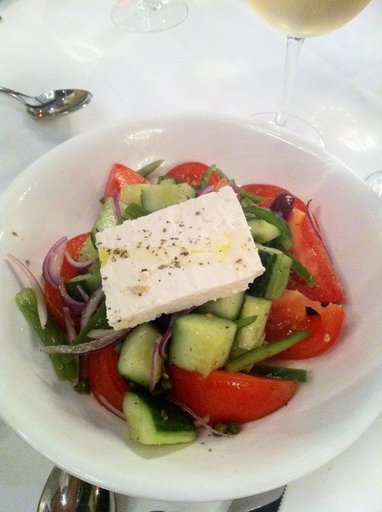
\includegraphics[width=3.33cm]{img/greekSaladFood101.jpg} }}%
        \qquad
        \subfloat[Pad Thaï]{{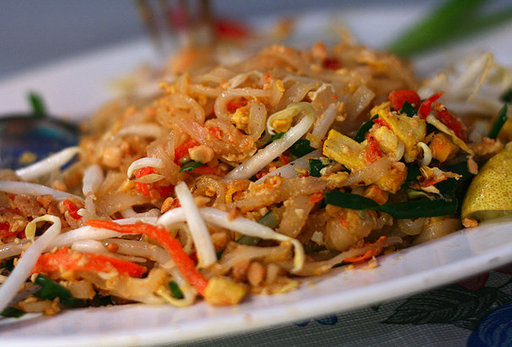
\includegraphics[width=3.33cm]{img/padThaiFood101.jpg} }}%
        \qquad
        \subfloat[Cheese Cake]{{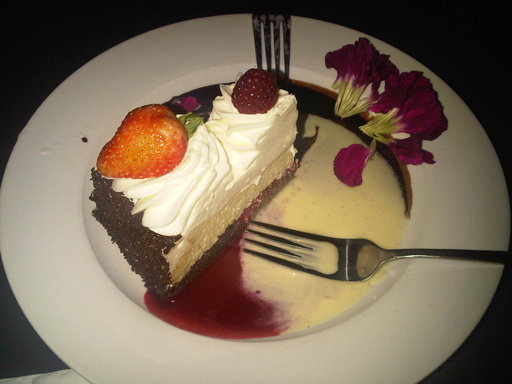
\includegraphics[width=3.33cm]{img/cheeseCakeFood101.jpg} }}%
        \caption{Exemple de photo du dataset}%
      \end{figure}%

      \subsection{Classe non-cookedDish}
      Pour cette classe je n'ai pas pu utiliser un dataset préexistant car aucun dataset ne se focalise sur "je ne suis pas un plat". Ma démarche a donc était totalement différente.
      \medbreak
      J'ai dans un premier temps classé en différentes catégories 3.000 images (fournie par Restofolio) qui avaient été manuellement rejeté par RestoFolio. De cette façon, j'ai pu voir les types d'images qui ne sont pas des plats les plus souvent ajoutés par les restaurateurs: photo de la salle du restaurant, de la carte/ardoise, publicité ou encore de matière première pour n'en citer que quelques uns.
      \medbreak
      J'ai ensuite peuplé ces différentes catégories à partir de petits dataset trouvés sur le web afin de rééquilibrer les deux classes. J'ai enfin ajouté deux dataset de contenus divers (et qui ne contiennent pas de photo de plat) afin de prévoir certaines classes oubliées.\footnote{Toutes les classes ainsi que les dataset utilisé peuvent être consultées directement sur un readme disponible sur le \href{https://github.com/plabadille/cookedDishRecognizer/blob/master/data-set/dataset_notCookedDish.txt}{github du projet}.}
      \medbreak
      \begin{figure}[!h]%
        \centering
        \subfloat[Légumes brut]{{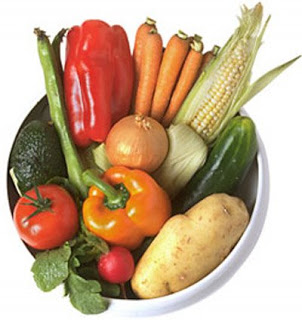
\includegraphics[width=3.33cm]{img/rawVegetablesNotCook.jpg} }}%
        \qquad
        \subfloat[Ardoise]{{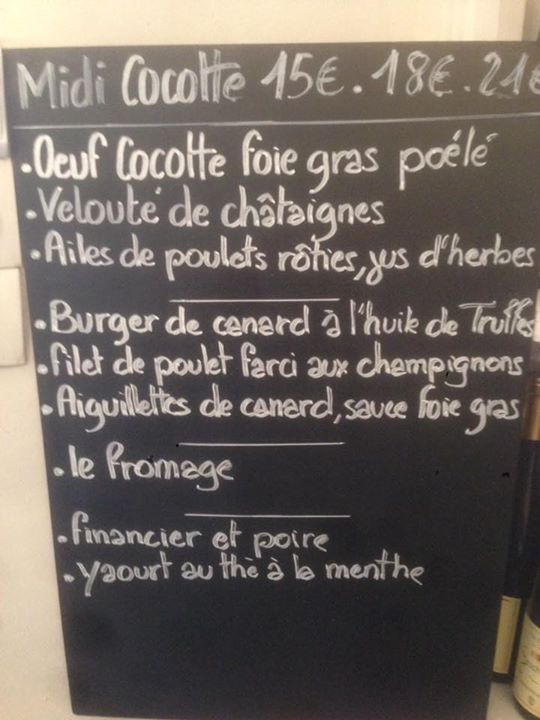
\includegraphics[width=3.33cm]{img/ardoiseNotCook.jpg} }}%
        \qquad
        \subfloat[Bouteilles de vin]{{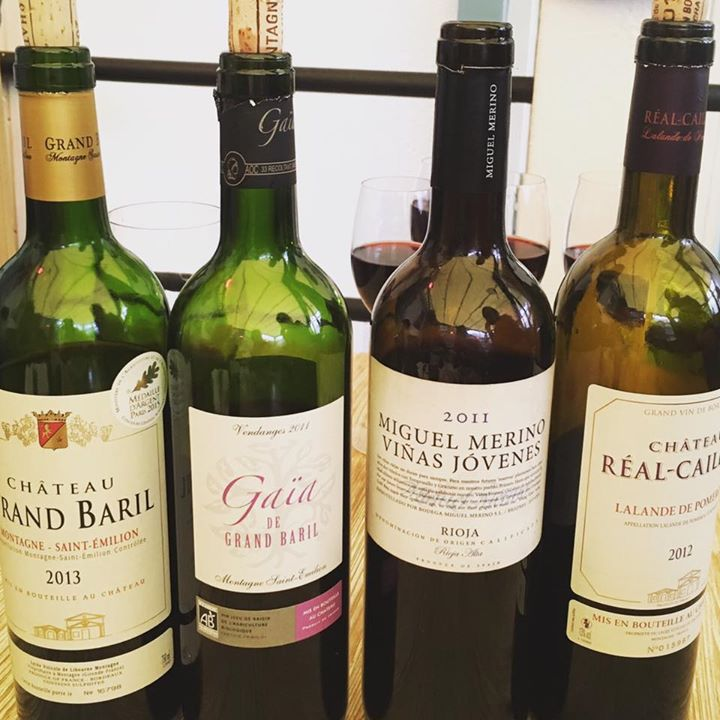
\includegraphics[width=3.33cm]{img/wineBottleNotCook.jpg} }}%
        \caption{Exemple de photo du dataset}%
      \end{figure}%

      \subsection{Préparation du set de données utilisé}
      Comme indiqué précédemment, le dataset de deux classes a été scindé en plusieurs sous-classe pour une utilité future. Pour le réseau actuel de neurones toutes les données doivent être dans le même dossier afin de faciliter leurs lectures.
      \medbreak
      J'ai donc établi une normalisation du dataset dans le dossier contenant les images nécessaires à l'entrainement et la validation: \textbf{<classe>\_<i>.jpg}. Renommer et déplacer 200.000 images réparties dans de multiples dossiers n'étant pas une option, j'ai opté pour la création d'un simple script bash:
      \begin{lstlisting}[language=Bash, title=mvIterator.sh]
      #!/bin/bash

      total=0
      for folder in *; do
          if [ $folder != *".sh" ]
              then
              i=0
              for img in ${folder}/*; do
                  ((i++))
                  mv ${img} ${folder}_${i}".jpg"    
              done
              ((total+=i))
          fi
      done
      echo "You have moved and rename $total files"
      \end{lstlisting}

    \section{Développement du modèle}
    Dans cette section je vais présenter les extraits principaux du code du modèle afin d'expliquer le fonctionnement du modèle et de chacune de ses spécificités. Le code original dans son intégralité est visualisable sur le \href{https://github.com/plabadille/cookedDishRecognizer/blob/master/cookedDishModel.py}{github du projet}. Veuillez noter qu'il existe deux versions du modèle et du système de prédiction: 
    \begin{itemize}
      \item La première ne peut être executée que dans un notebook Jupyter et permet d'avoir des indicateurs visuels sur les résultats du modèle.
      \item La seconde peut être executée directement en console (dans un environnement Tensorflow) mais ne donnera que des informations textuelles sur le modèle.
    \end{itemize}

      \subsection{Le modèle (cookedDishModel.py)}
      Tout d'abord, je souhaite préciser que la base de ce code ne vient pas de moi. J'ai pris modèle sur un \href{https://www.kaggle.com/vshevche/dogs-vs-cats-redux-kernels-edition/catdognet-keras-convnet-starter/run/790364}{Convnet starter} de Jeff Delanay, lui-même fortement inspiré du tutoriel \href{https://blog.keras.io/building-powerful-image-classification-models-using-very-little-data.html}{Building powerful image classification models using very little data} de Francois Chollet.
      \medbreak
      Les différences principales avec ces deux modèles sont indiquées en commentaire dans le code au début du script. Globalement, j'ai fais du refactoring, adapté le modèle au besoin et ajouté plusieurs améliorations que je vais vous présenter maintenant (une cross validation par exemple).
      \bigbreak

      Dans un premier temps, le script importe les dépendances du modèle puis on va stocker la localisation des images en numpy array\footnote{Table d'index sous forme de tableau multidimensionnel (ici 3d)} afin de pouvoir les apprendre au modèle. Ces images vont ensuite être redimensionnées (le modèle a besoin d'avoir des images de la même taille) et converties afin que le modèle puisse la comprendre.
      \medbreak
      C'est après que la logique binaire de notre modèle va prendre naissance, le snippet suivant montre comment l'on assigne chaque image à ça classe respective:
      \begin{lstlisting}[title=cookedDishModel.py (l.96)]
      labels = []
      for i in train_images:
        if 'cookedDish' in i:
          labels.append(1)
        else:
      labels.append(0)
      \end{lstlisting}
      \medbreak
      On va ensuite définir notre modèle. Un modèle est composé de différentes couches. Dans le cas présent, notre modèle est une version réduite de l'architecture VGG16\footnote{architecture VGG16: réseau à 16 couches utilisés par l'équipe VGG pour la compétition ILSVRC-2014 competition. Cf \href{https://arxiv.org/abs/1409.1556}{Very Deep Convolutional Networks for Large-Scale Image Recognition}}
      \medbreak
      Dans notre cas vous pouvez voir l'utilisation de quatre blocs convolutionnels\footnote{Cf \href{https://cs231n.github.io/convolutional-networks/\#conv}{Convolutional Layer}} ainsi qu'un "fully-connected" classifieur\footnote{Cf \href{https://cs231n.github.io/convolutional-networks/\#fc}{Fully-connected layer}}. Grossièrement, chaque couche convenlutionelle n'a accès qu'aux couches inférieures: l'apprentissage du modèle passe par elles (on dit qu'elles sont connectées localement). La couche "fully-connected", elle, a accès à tout le modèle: c'est par elle que sont faites les prédictions après la période d'apprentissage. Enfin l'optimisateur et l'objectif sélectionné sont préconisés pour les modèles de classification binaire.

      \begin{lstlisting}[title=cookedDishModel.py (l.133)]
      optimizer = RMSprop(lr=1e-4)
      objective = 'binary_crossentropy'

      def isPlat():
        model = Sequential()

        model.add(Convolution2D(32, 3, 3, border_mode='same', input_shape=(3, ROWS, COLS), activation='relu'))
        model.add(Convolution2D(32, 3, 3, border_mode='same', activation='relu'))
        model.add(MaxPooling2D(pool_size=(2, 2), dim_ordering="th"))

        model.add(Convolution2D(64, 3, 3, border_mode='same', activation='relu'))
        model.add(Convolution2D(64, 3, 3, border_mode='same', activation='relu'))
        model.add(MaxPooling2D(pool_size=(2, 2), dim_ordering="th"))
        
        model.add(Convolution2D(128, 3, 3, border_mode='same', activation='relu'))
        model.add(Convolution2D(128, 3, 3, border_mode='same', activation='relu'))
        model.add(MaxPooling2D(pool_size=(2, 2), dim_ordering="th"))
        
        model.add(Convolution2D(256, 3, 3, border_mode='same', activation='relu'))
        model.add(Convolution2D(256, 3, 3, border_mode='same', activation='relu'))
        model.add(MaxPooling2D(pool_size=(2, 2), dim_ordering="th"))

        model.add(Flatten())
        model.add(Dense(256, activation='relu'))
        model.add(Dropout(0.5))
        
        model.add(Dense(256, activation='relu'))
        model.add(Dropout(0.5))

        model.add(Dense(1))
        model.add(Activation('sigmoid'))

        model.compile(loss=objective, optimizer=optimizer, metrics=['accuracy', 'recall', 'precision'])
        return model

      model = isPlat()
      \end{lstlisting}

      \medbreak
      Le petit bout de code ci-dessous va permettre d'appliquer la méthode de "cross validation" lors de l'apprentissage. Cela signifie qu'à chaque nouvelle epoch,\footnote{Un epoch correspond à un cycle complet d'apprentissage (toutes les données sont passées au moins une fois)} le jeu d'apprentissage et le jeu de validation va être modifié de façon aléatoire (définie par l'attribut "random\_state").
      \begin{lstlisting}[title=cookedDishModel.py (l.175)]
      X_train, X_test, y_train, y_test = train_test_split(train, labels, train_size=VALIDATION_PERCENT, random_state=RANDOM_STATE)
      \end{lstlisting}

      \medbreak
      Cette petite classe est indispensable pour avoir des statistiques précises sur l'apprentissage de notre modèle. Grâce à une callback, elle nous permet de récupérer des informations sur les performances de notre modèle à chaque epoch. Les attributs préfixés par "val\_" correspondent aux statistiques de validation, les autres à l'apprentissage.
      \begin{lstlisting}[title=cookedDishModel.py (l.177)]
      class trendsHistory(Callback):
        def on_train_begin(self, logs={}):
          self.losses = []
          self.val_losses = []
          self.acc = []
          self.val_acc = []
              
        def on_epoch_end(self, batch, logs={}):
          self.losses.append(logs.get('loss'))
          self.val_losses.append(logs.get('val_loss'))
          self.acc.append(logs.get('acc'))
          self.val_acc.append(logs.get('val_acc'))
      \end{lstlisting}

      \medbreak
      L'avantage de permettre à un modèle de parcourir plus d'une epoch est qu'il améliore ça capacité à généraliser et devient plus performant réduisant ainsi ce que la losses\footnote{somme des carrés résiduels des erreurs du modèle} du modèle. Cependant après un certain temps le modèle va commencer à trop généraliser et cette accumulation de données va alors inverser cette tendance. La fonction ci-dessous permet d'arrêter le modèle avant le nombre d'epoch prédéfini dans le cas où la losses de validation ne diminue plus. Elle est accompagnée d'un délai afin de se prémunir de fausses alertes.
      \begin{lstlisting}[title=cookedDishModel.py (l.191)]
      ## Early stopping if the validation loss doesn't decrease anymore
      early_stopping = EarlyStopping(monitor='val_loss', patience=EARLY_SOPPING_PATIENCE, verbose=1, mode='min')
      \end{lstlisting}

      \medbreak
      Enfin, cette fonction permet de sauvegarder le modèle à chaque fois que la losses de validation s'améliore (vérification à la fin de chaque epoch). Cette fonction permet de toujours conserver la meilleure version du modèle malgré le délai de fin prématurée que nous venons de voir.
      \begin{lstlisting}[title=cookedDishModel.py (l.194)]
      ## We just save the best model, not the last one used
      filepath = SAVE_MODEL_DIR + SAVE_MODEL_WEIGHT_NAME
      model_checkpoint = ModelCheckpoint(filepath=filepath, monitor='val_loss', save_best_only=True, verbose=1, mode='min', save_weights
      \end{lstlisting}

      \subsection{Le système de prédiction (demo.py)}
      Cette partie est beaucoup simple, dans un premier temps on va simplement recharger notre modèle à partir de deux fichiers de sauvegarde générés à la fin de l'apprentissage: les métadata de notre modèle contenues dans un fichier json et les weights du modèle contenus dans un fichier hdf5.
      \begin{lstlisting}[title=test.py (l.32)]
      json_file = open(SAVE_MODEL_DIR + SAVE_MODEL_JSON_NAME, 'r')
      loaded_model_json = json_file.read()
      json_file.close()

      model = model_from_json(loaded_model_json)
      model.load_weights(SAVE_MODEL_DIR + SAVE_MODEL_WEIGHT_NAME)
      \end{lstlisting}

      \medbreak
      La démo proposée par ce script est automatisée: la seule chose à faire est de placer les images à tester dans le dossier défini par la constante PREDICT\_DIR. Les prédictions sont ensuite modélisées pour indiquer la probabilité correspondant à la prédiction. Comme vous pouvez le voir, le modèle ne s'interesse pas vraiment à la classe "something else", il nous retournera toujours des statistiques pour notre classe principale. Si ces statistiques sont inférieures à 50\% c'est que le modèle pense que la photo proposée appartient à l'autre classe.
      \begin{lstlisting}[title=test.py (l.194)]
      test_images =  [PREDICT_DIR+i for i in os.listdir(PREDICT_DIR)]
      test, count = prep_data(test_images)
      predictions = model.predict(test, verbose=0)

      for i in range(0,count):
        print("\n" + "Image " + path_image[i] + ":")
        if predictions[i, 0] >= 0.5: 
          print('I am {:.2%} sure this is a cooked dish'.format(predictions[i][0]))
        else: 
          print('I am {:.2%} sure this is something else'.format(1-predictions[i][0]))
      \end{lstlisting}


  \chapter{Choix du modèle, performances et analyse}

    \section{Mise en garde}
    Attention, l'entrainement de ce modèle nécessite au minimum 6Go de mémoire vive disponible. L'entrainement du modèle a pris 40 minutes (dont 10 minutes de chargement d'image) avec deux NVDIA-970GTX. Exécuter ce modèle via le processeur prendrait environ 4 à 6 heures en CPU.

    \begin{figure}[!h]%
      \centering
      \subfloat[Specs durant le training]{{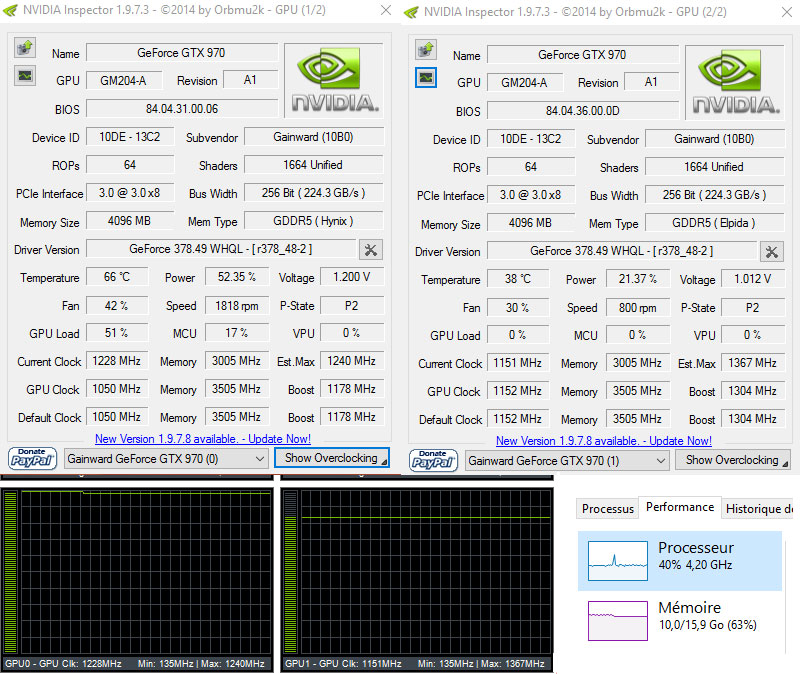
\includegraphics[width=15cm]{img/spec.jpg} }}%
    \end{figure}%

    \section{Choix du modèle}    
      Dans cette section je vais tâcher de montrer mon raisonnement pour mon choix final du modèle. J'ai sélectionné les quatre exemples qui ont fait avancer mon raisonnement mais sachez que j'ai généré environ 20 modèles différents pour trouver un modèle satisfaisant.
      \medbreak
      Mon choix c'est fait en trois étapes correspondant aux trois sous-sections ci-dessous: l'analyse de l'accuracy\footnote{accuracy: mesure à quelle fréquence le modèle choisit la bonne classe}/losses, l'analyse des courbes ROC et enfin l'analyse des prédictions de test.
      \medbreak
      Vous pouvez voir ci-dessous de quelle façon le modèle perçoit les deux classes: 
      \begin{figure}[!h]%
        \centering
        \subfloat[Plat cuisiné moyen]{{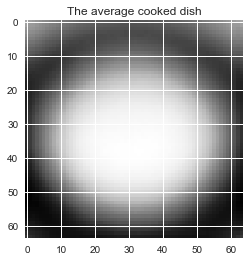
\includegraphics[width=5cm]{img/averageDish.png} }}%
        \qquad
        \subfloat[Autre chose moyen]{{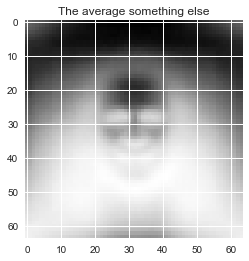
\includegraphics[width=5cm]{img/averageElse.png} }}%
        \qquad
        \caption{Classe vue par le modèle}%
      \end{figure}%
      \bigbreak
      Enfin, pour s'y retrouver facilement, j'ai nommé chaque modèle de A à D de façon chronologique (le modèle A est le premier modèle que j'ai entrainé). Les différences entre ces modèles sont principalement des différences de taille de batch\footnote{Batch size: nombre de données propagées dans le réseau: permet de calculer le nombre d'itérations nécessaires par epoch.} et le pourcentage de données utilisées pour la validation:
      \begin{itemize}
        \item Modèle A: batch size = 16, validation = 35\%
        \item Modèle B: batch size = 50, validation = 35\%
        \item Modèle C: batch size = 50, validation = 45\%
        \item Modèle D: batch size = 60, validation = 45\%
      \end{itemize}

      \subsection{Accuracy et Losses par epoch}
      Les premiers indicateurs auxquels je me suis intéressé pour le choix de mon modèle sont l'accuracy et la losses. Ils permettent de voir les performances du modèle, mais leur évolution par epoch est encore plus intéressante. C'est par le biais de cette évolution que l'on peut vérifier que le modèle n'entre pas dans un état d'overfitting\footnote{Le modèle connait trop bien le jeu de donnée d'entrainement impactant son habilité à généraliser.} ou d'underfitting\footnote{Le modèle n'arrive pas à généraliser (entrainement, validation et prédiction)} (problème de généralisation du modèle).
      \medbreak
      \begin{figure}[!h]%
        \centering
        \subfloat[Modèle A]{{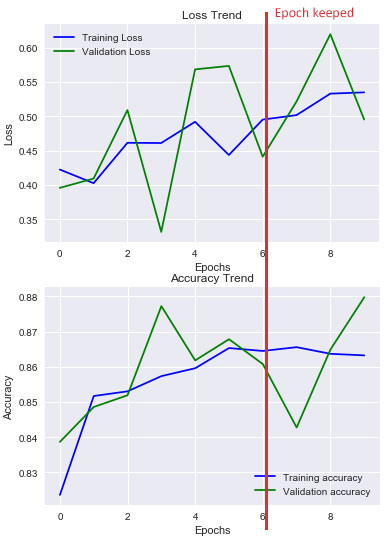
\includegraphics[width=7cm]{img/1-accLoss.jpg} }}%
        \qquad
        \subfloat[Modèle B]{{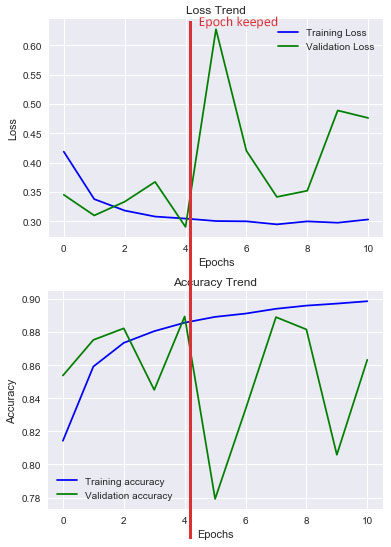
\includegraphics[width=7cm]{img/2-accLoss.jpg} }}%
        \qquad
        \subfloat[Modèle C]{{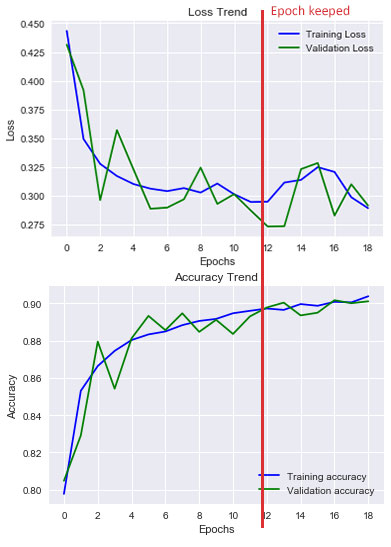
\includegraphics[width=7cm]{img/3-accLoss.jpg} }}%
        \qquad
        \subfloat[Modèle D]{{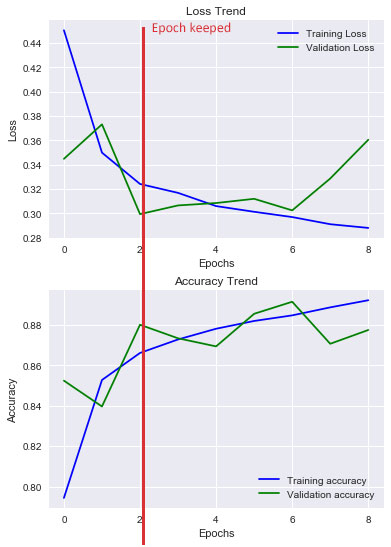
\includegraphics[width=7cm]{img/4-accLoss.jpg} }}%
        \caption{Accuracy and losses}%
      \end{figure}%
      \FloatBarrier
      \bigbreak
      Pour interpréter ces résultats (attention aux échelles, elles sont dynamiques en fonction des valeurs) je me suis basé sur ce modèle:
      \begin{itemize}
        \item Underfitting: Les erreurs de validation et d'apprentissage sont élevées (Losses élevé et accuracy basse).
        \item Overfitting: Les erreurs de validation sont élevées alors que les erreurs d'apprentissage sont faibles.
        \item Bon ajustement: Les erreurs de validation sont faibles mais légèrement supérieures aux erreurs d'apprentissages
        \item Ajustement inconnu: Les erreurs de validation sont faibles mais les erreurs d'apprentissage sont "élevées".
      \end{itemize}
      \bigbreak
      Dans un premier temps, on remarque que les modèles A et B sont très instables: on constate des pics importants sur la validation. Cette dernière est globalement éloignée des valeurs de validation ce qui n'est pas une bonne chose (elle devrait être légèrement supérieure pour la losses et inférieure pour l'accuracy). Ces modèles oscillent selon les epochs entre overfitting et un ajustement inconnu.
      \medbreak
      Les deux autres modèles (C et D) ont des courbes beaucoup plus cohérentes (validation proche de l'apprentissage) et semblent donc plus pertinent. Le modèle C est conservé en epoch 12 alors que le modèle D a atteind ses meilleures performances dès l'epoch 2. Cette information couplée au fait que le modèle C n'a pas connu de cas flagrant d'overfitting (léger pic pendant l'epoch 2 mais la différence n'est que de 0.035 environ) semblerait donc être pour le moment le plus pertinent.
      \smallbreak
      Notons que ces légers pics ne traduisent pas forcément de l'overfitting: le modèle utilisant une cross validation, il est tout à fait possible que les données de validation soient plus complexes à résoudre que les données d'apprentissage.
      \medbreak
      Quoi qu'il en soit, le modèle C et le modèle D rentre dans le cas "d'ajustement inconnu", il faudra donc analyser les courbes ROC et les prédictions de ces modèles afin de les départager et être sûr qu'ils sont efficaces.

      \subsection{Courbe ROC}
      La courbe ROC (Receiving Operating Characteristics) est une représentation graphique des performances d'un modèle. En ordonnée, on trouve la sensibilité (Le taux de vrai positif) et en abscisse, l'inverse de la spécificité (1- taux de faux positif). Comme le montre l'exemple d'interprétation suivant, plus la courbe se situe "haut" dans le graphique, plus le modèle est performant:
      \medbreak
      \begin{figure}[!h]%
        \centering
        \subfloat[Interprétation courbe ROC]{{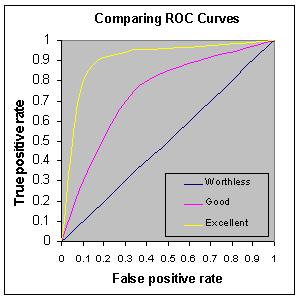
\includegraphics[width=6cm]{img/roccomp.jpg} }}%
      \end{figure}%
      \bigbreak
      Notons enfin que ces courbes correspondent aux taux d'erreurs de l'epoch retenus par le modèle.
      \medbreak
      \begin{figure}[!h]%
        \centering
        \subfloat[Modèle A]{{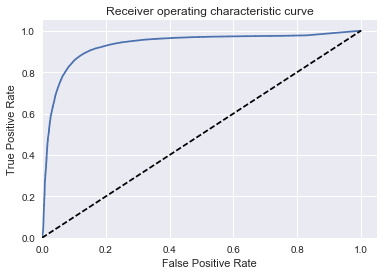
\includegraphics[width=7cm]{img/1-roc.png} }}%
        \qquad
        \subfloat[Modèle B]{{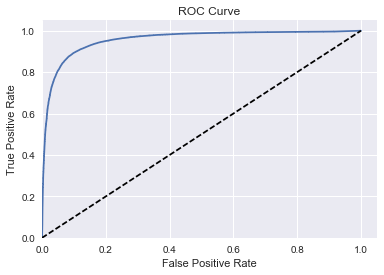
\includegraphics[width=7cm]{img/2-roc.png} }}%
        \qquad
        \subfloat[Modèle C]{{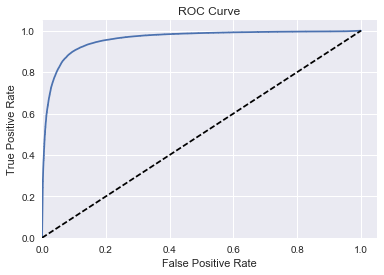
\includegraphics[width=7cm]{img/3-roc.png} }}%
        \qquad
        \subfloat[Modèle D]{{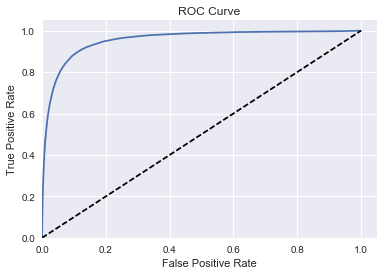
\includegraphics[width=7cm]{img/4-roc.png} }}%
        \caption{Courbes ROC}%
      \end{figure}%
      \FloatBarrier
      \bigbreak
      Bien que les courbes des modèles A et B soient très légèrement moins bonnes, elles sont toutes excellentes. Cela ne veut bien entendu pas dire que notre modèle est parfait mais traduit une bonne performance de tous nos modèles.
      \medbreak
      Si un mauvais modèle (établissant de mauvaise prédiction) a malgré tout une courbe ROC excellente, cela signifi que le modèle (hardcode) est bon mais que le jeu de donnée d'une ou des deux classes n'est pas adapté.
      \medbreak
      Nous ne pouvons donc rien conclure de cette courbe ROC avant d'avoir analysé les performances de prédiction des modèles, si ce n'est que le "code" de notre modèle est bon.

      \subsection{Prédiction}
      Pour valider mon modèle à partir des prédictions (faites sur le modèle complètement entrainé), j'ai soigneusement choisi quatre images de plats et quatre images qui n'en sont pas.
      \medbreak
      \begin{figure}[!h]%
        \centering
        \subfloat[Item 1]{{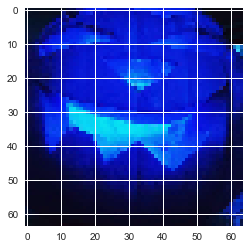
\includegraphics[width=3cm]{img/output_0_15.png} }}%
        \qquad
        \subfloat[Item 2]{{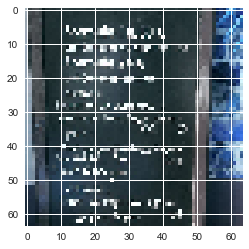
\includegraphics[width=3cm]{img/output_0_19.png} }}%
        \qquad
        \subfloat[Item 3]{{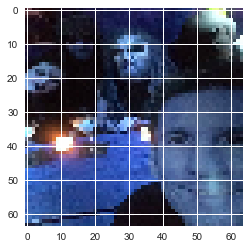
\includegraphics[width=3cm]{img/output_0_17.png} }}%
        \qquad
        \subfloat[Item 4]{{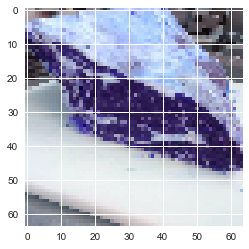
\includegraphics[width=3cm]{img/output_0_21.png} }}%
        \caption{Prédictions (classe autre chose)}%
      \end{figure}%
      \FloatBarrier
      \bigbreak

      \begin{table}[!h]
      \centering
        \begin{tabular}{lllll}
          \hline
          Modèle & Item 1 & Item 2 & Item 3 & Item 4 \\
          \hline
          A & 100\% & 98.39\% & -67.06\% & -69.09\% \\
          B & 98.73\% & 100\% & 50.49\% & -97.84\% \\
          C & 99.92\% & 99.94\% & -90.12\% & 68.02\% \\
          D & -81.84\% & 99.91\% & -99.41\% & -98.77\% \\
          \hline
        \end{tabular}
      \end{table}
      \smallbreak

      \medbreak
      \begin{figure}[!h]%
        \centering
        \subfloat[Item 5]{{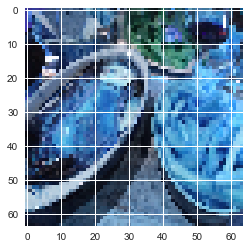
\includegraphics[width=3cm]{img/output_0_23.png} }}%
        \qquad
        \subfloat[Item 6]{{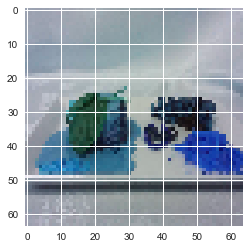
\includegraphics[width=3cm]{img/output_0_25.png} }}%
        \qquad
        \subfloat[Item 7]{{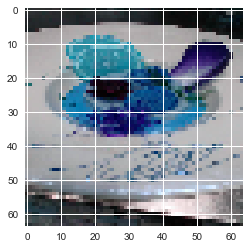
\includegraphics[width=3cm]{img/output_0_27.png} }}%
        \qquad
        \subfloat[Item 8]{{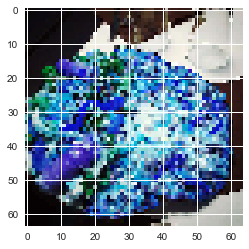
\includegraphics[width=3cm]{img/output_0_29.png} }}%
        \caption{Prédictions (classe plat cuisiné)}%
      \end{figure}%
      \FloatBarrier
      \smallbreak

      \begin{table}[!h]
      \centering
        \begin{tabular}{lllll}
          \hline
          Modèle & Item 5 & Item 6 & Item 7 & Item 8 \\
          \hline
          A & 89.80\% & 63.06\% & 99.59\% & 99.65\% \\
          B & 89.69\% & -58.22\% & 99.71\% & 97.32\% \\
          C & 87.32\% & 57.96\% & 99.48\% & 96.58\% \\
          D & 97.96\% & 92.77\% & 99.89\% & 99.69\% \\
          \hline
        \end{tabular}
      \end{table}
      \medbreak
      Il faut tout d'abord noter que les valeurs négatives correspondent à une erreur. Dans un premier temps, on peut exclure le modèle D: il est beaucoup trop confiant (rarement moins de 97\% de certitude) et choisi presque toujours un plat.
      \medbreak
      Le modèle A, lui, échoue à la différenciation des deux "autres" les plus complexes ce qui le rend moins intéressant que les autres.
      \medbreak
      Enfin, le modèle B est le seul à différencier les visages de justesse mais il se trompe dans l'analyse du plat le plus complexe. Ainsi, le modèle C semble être le pertinent: il est d'ailleurs le seul modèle parmi tous mes essais (une vingtaine) à avoir choisi la bonne classe pour la pièce de viande brute. De plus, ses seuils de confiances affichés sont cohérents avec la difficulté de classification des images données.
      \medbreak
      Il faut bien garder à l'esprit que plusieurs de ces images ici sont difficiles. J'ai testé chaque modèle sur des photos plus classiques et le modèle B et C s'en sortent très bien (D est catastrophique: il indique quasiment toujours un plat).

      \subsection{Sélection du meilleur modèle}
      En mettant bout à bout chacune de ces trois analyses pour chacun des modèles, j'ai décidé de sélectionner le modèle C qui est toujours le plus pertinent à chaque étape. Le modèle B était également intéressant mais son instabilité (accuracy et losses) est préoccupante.
      \medbreak
      Je souhaite tout de même indiquer que je pense qu'un travail sur le jeu de données serait utile pour obtenir un modèle plus performant. La courbe ROC est une preuve de performance du modèle mais les prédictions indiquent que ce modèle pourrait encore être amélioré. Je n'ai malheureusement pas eu le temps de remanier ce dernier (les dataset sont gros et celà nécessite beaucoup d'analyse et de temps de calculs) mais je pense que le modèle C reste très satisfaisant.

  \chapter{Conclusion}

    \section{Présentation des améliorations possibles}
    Faute de temps et du défi que représentais ce projet, je n'ai pas pu aller aussi loin que prévu. J'avais néanmoins effectué des recherches préliminaires sur plusieurs points que je souhaite exposer brièvement.

      \subsection{Implémentation dans un environnement tensorflow "less"}
      Actuellement le modèle est fonctionnel est peu établir des prédictions à la demande. Il n'est néanmoins pas exploitable à l'exterieur de son environnement complexe ce qui le relègue à l'état d'experimentation alors qu'il pourrait devenir un véritable outil. 
      \medbreak
      Voici les différentes solutions pour utiliser ce modèle pré-entrainé à partir d'une autre application n'évoluant pas dans un environnement approprié:
      \begin{itemize}
        \item \href{https://github.com/transcranial/keras-js/blob/master/README.md}{Keras-js}: permet la création d'une application en VueJs pouvant charger le modèle directement dans le navigateur puis effectuer des prédictions à la demande.
        \item \href{https://www.tensorflow.org/deploy/tfserve}{TensorFlow Serving}: permets d'installer le réseau de neurones sur un serveur dans son environnement pour ensuite retourner des prédictions par le biais d'une API.
        \item \href{https://github.com/riga/tfdeploy}{TfDeploy}: permet d'exporter un réseau de neurones pré-entrainé directement dans une application python par le biais de numpy.
      \end{itemize}

      \subsection{Du modèle binaire vers un modèle multi-classe}
      Après une longue période de réflexion sur le sujet, je pense que transformer ce modèle binaire en modèle multi-classe n'est pas la solution pour labéliser chaque plat. En rajoutant des classes ont va également diminuer l'habilité de notre modèle à différencier un plat d'autre chose. Cela étant, au vu de notre problème de départ, je ne pense pas qu'il soit avisé de partir dans cette direction. 
      \medbreak
      Cependant, je pense qu'il est également possible d'effectuer une labélisation sans déteriorer la qualité de la différenciation binaire: créer un second modèle. En effet, si le premier modèle binaire épure déjà les photos qui ne sont pas des plats, le second modèle pourra alors se focaliser sur la labélisation.

    \section{Problèmes rencontrés}
    Le premier problème majeur que j'ai rencontré est lié au fait que je me suis lancé dans ce projet avec absolument aucune connaissance en deep learning (ou même big data d'ailleurs) et réseaux de neurones automatisés. Ces lacunes ont entrainé des problèmatiques majeures quant à la compréhension du fonctionnement de cette technologie et du vocabulaire relatif à son utilisation. Il n'existe pas de "tutoriel du zero" dans le monde du deep learning et même les exemples les plus simples peuvent paraître totalement abstraits.
    \medbreak
    J'ai ensuite eu beaucoup de mal à installer l'environnement adéquate afin de pouvoir commencer à tester des modèles: j'ai mis trois jours à créer un environnement de travail fonctionnel. J'ai néanmoins fini par trouver une procédure plutôt simple et je suis désormais capable de réinstaller cet environnement sur windows et linux.
    \medbreak
    Enfin, le temps et la quantité de données à traiter a souvent été problématique: 10Go de data-set, 40 minutes par entrainement de modèle (sans compter les nombreux modèles qui ont buggé après 30mm de calculs durant la phase de développement).

    \section{Feedback}
    Quand j'ai choisi ce projet, je ne m'attendais absolument pas à développer un modèle de réseau de neurones. Ce projet tuteuré a été mon plus gros défi en matière de développement et j'ai plus d'une fois cru que je n'arriverais pas à le terminer dans les délais impartis étant donnée sa complexité (et mon manque d'expérience dans ce domaine).
    \medbreak
    Malgré tout, travailler sur ce projet a été un véritable plaisir, ainsi qu'une bonne opportunité de découvrir et d'apprivoiser la puissance du deep learning. Je pense sincèrement que ce n'est pas la dernière fois que je vais travailler sur un modèle de ce genre et je pense qu'ils vont devenir de plus en plus présents dans le monde du web.    

    \section{Remerciements}
    Tout d'abord je tiens à sincèrement remercier François Rioult qui m'a encadré sur ce projet pour m'avoir conseillé et rassuré dans les moments de doutes.
    \medbreak
    Marc Houssaye pour m'avoir proposé ce sujet et ainsi donné, sans le savoir, l'opportunité de découvrir la puissance des systèmes de réseaux de neurones automatisés.
    \medbreak
    Frederic Jurie et Alexis Lechervy pour m'avoir indiqué des solutions/choix de départ, c'est grâce à leur expertise que j'ai pu démarrer ce projet.
    \medbreak
    Le Master DNR2i de l'Université de Caen Normandie pour m'avoir permis de suivre cette formation sans expérience de développement préliminaire.
    
    \newpage

    \section{Sources}
    Voici un extrait des sources principales qui m'ont permis de développer ce projet:

      \subsection{Littérature et documentation}
      \begin{itemize}
        \item \href{http://xenon.stanford.edu/~pgolle/papers/dogcat.pdf}{Machine Learning Attacks Against the Asirra CAPTCHA} de Philippe Golle (Palo Alto Research Center).
        \item \href{https://arxiv.org/abs/1409.1556}{Very Deep Convolutional Networks for Large-Scale Image Recognition} de Karen Simonyan et Andrew Zisserman
        \item \href{https://cs231n.github.io/convolutional-networks/}{Convolutional Neural Networks (CNNs / ConvNets)} de la Stanford CS class
        \item \href{https://deeplearning4j.org/glossary}{Deep Learning and Neural Network Glossary} de deeplearning4j
        \item \href{http://webia.lip6.fr/~cord/pdfs/publis/CordCooking2015icme.pdf}{RECIPE RECOGNITION WITH LARGE MULTIMODAL FOOD DATASET} de Xin Wang, Devinder Kumar, Nicolas Thome, Matthieu Cord et Frédéric Precioso.
        \item \href{https://arxiv.org/pdf/1510.02078v1.pdf}{Leveraging Context to Support Automated Food Recognition in Restaurants} de Vinay Bettadapura, Edison Thomaz, Aman Parnami, Gregory D. Abowd et Irfan Essa
        \item \href{https://arxiv.org/pdf/1604.07953v2.pdf}{Simultaneous Food Localization and Recognition} de Marc Bolanos et Petia Radeva
        \item \href{https://arxiv.org/pdf/1612.06543v1.pdf}{Wide-Slice Residual Networks for Food Recognition} de Niki Martinel, Gian Luca Foresti et Christian Micheloni
        \item \href{https://keras.io/}{documentation Keras}
        \item \href{https://www.tensorflow.org/get\_started/get\_started}{documentation Tensorflow}
        \item \href{https://www.kaggle.com/wiki/Home}{documentation Kaggle }
      \end{itemize}

      \subsection{Data-set}
      \begin{itemize}
        \item \href{http://vis-www.cs.umass.edu/lfw/}{lfw face data-set}
        \item \href{http://web.mit.edu/torralba/www/indoor.html}{Indoor Scene Recognition data-set}
        \item \href{https://graphics.cs.msu.ru/en/research/projects/msr/geometry}{EurasianCitiesBase data-set}
        \item \href{http://cvcl.mit.edu/database.htm}{Visual Cognition Laboratory data-set}
        \item \href{https://www.csc.kth.se/~heydarma/Datasets.html}{KTH-ANIMALS data-set} 
        \item \href{https://www.kaggle.com/c/dogs-vs-cats-redux-kernels-edition}{dogsVsCats data-set}
        \item \href{https://www.vision.caltech.edu/Image_Datasets/Caltech256/}{Caltech256 data-set}
        \item \href{http://host.robots.ox.ac.uk/pascal/VOC/voc2007/index.html}{voc2007 data-set}
        \item \href{http://press.liacs.nl/mirflickr/mirdownload.html}{mirflickr data-set}
        \item \href{https://www.vision.ee.ethz.ch/datasets_extra/food-101/}{ETHZ-Food-101 data-set}
      \end{itemize}
          
\end{document}
